%%
%% if lualatex is not used, compile to PDF 1.4 (compatibility to Adobe Acrobat)
%%
\RequirePackage{ifluatex}
\ifluatex
\else
	\RequirePackage{pdf14}
\fi

\documentclass[aspectratio=1610]{beamer}
%%
%% E.ON ERC Beamer Theme (layout based on E.ON ERC PowerPoint template)
%% by Simon Pickartz, Institute for Automation of Complex Power Systems, 2014
%%   spickartz@eonerc.rwth-aachen.de 
%% based on RWTH Latex template 
%% by Georg Wassen, Lehrstuhl für Betriebssysteme, 2013
%%    wassen@lfbs.rwth-aachen.de
%%
%% The templates are derived from the beamer documentation and the provided 
%% templates, hence, the same licence applies:
%%
%% ----------------------------------------------------------------
%% |  This file may be distributed and/or modified                |
%% |                                                              |
%% |  1. under the LaTeX Project Public License and/or            |
%% |  2. under the GNU Public License.                            |
%% |                                                              |
%% |  See the file doc/licenses/LICENSE for more details.         |
%% ----------------------------------------------------------------
%%
%% Version 0.1    03/28/2014    Initial presentation using this theme
%% Version 0.2    04/01/2014    First version to be published in the institute 
%%

\usepackage{ifthen}

% Whether to output the Print version (with RWTH logo) or the public version
\newboolean{outputPrintVersion}
\setboolean{outputPrintVersion}{false}

\usepackage[]{luainputenc}                 
\usepackage[english]{babel}
\usetheme[]{eonerc}

\usepackage[T1]{fontenc} 					% Font encoding
\usepackage{lmodern} 						% Select Linux Modern Fonts
\usepackage{graphicx} 						% needed to include graphics
\beamertemplatenavigationsymbolsempty 		% Disable navigation symbols

\usepackage{listings}
\usepackage{tikz}

\usetikzlibrary{calc,positioning,fit,matrix,shadows,chains,arrows,shapes,spy,fadings,shadings}
\usepackage{pgfplots}
\usetikzlibrary{pgfplots.units,shapes.symbols,shapes.arrows}

\tikzset{
	cf_base/.style={font=\sffamily\footnotesize, node distance=12mm, fill=white},
	cf_block/.style={cf_base, draw, rectangle, rounded corners, on grid, align=center},
	cf_data/.style={cf_base, draw, cylinder, aspect=0.2, on grid, shape border rotate=90]},
	cf_head/.style={font=\sffamily\bfseries\normalsize, on grid},
	cf_impl/.style={cf_base, fill=yellow!40},
	cf_label/.style={align=left, draw opacity=0, font=\sffamily\tiny},
	cf_line/.style={cf_base, draw=black, -latex},
	cf_skiplistitem/.style={cf_base, draw, rectangle split, rectangle split parts=#1, rectangle split empty part height=1.3ex, rectangle split empty part width=1ex, align=center},
	cf_onslide/.code args={<#1>#2}{\only<#1>{\pgfkeysalso{#2}}},
	cf_emphline/.style={line width=0.8pt},
	cf_blackbox/.style={cf_base, draw, rectangle, on grid, align=center, color=white, fill=black, minimum height=25mm, minimum width=50mm}
}

\definecolor{windows_gray}{RGB}{212,208,200}
\definecolor{windows_blue}{RGB}{10,36,106}

\newcommand\myheading[1]{{\Large\bfseries#1}\par\bigskip}


%%%%%%%%%%%%%%%%%%%%%%%%%%%%%%%%%%%%%
%% configure title page and author information
%%-------------------------------
%% You can always provide a short version: \title[short]{long title}
%%   title        -- Title of the presentation
%%                   The title appears on the first page and may contain 
%% 					 a line break: \\ 
%%                   The short title appears in the footer line
%%   subtitle     -- Appears below the title
%%   titlegraphic -- Currently not supported
%%   author       -- Name of the author(s)
%%   email        -- E-Mail address of author (optional)
%%   institute    -- Name of the institution (e.g. chair)
%%   webaddress   -- Web address (default is www.rwth-aachen.de), 
%% 					 (see slide generated with \lastpage)
%%   date         -- Date of the presentation 
%% 					 (or use \date to insert the date of the PDF generation)
%%   subject      -- This is only for the PDF meta data
%%   keywords     -- This is only for the PDF meta data
%%   logo         -- Logo, don't change (given by coporate identity templates)
\title[Printing Stack for the ReactOS Operating System]{Analysis, Design and Implementation of a Printing Stack \\for the Open-Source ReactOS Operating System}
\titlebanner{pictures/title_small}
\subtitle{Bachelor Thesis Presentation}
\author{Colin Finck}
\email{colin.finck@rwth-aachen.de} 							% optionally
\institute[ACS]{Automation of Complex Power Systems}
\webaddress{www.eonerc.rwth-aachen.de} 						% overrides rwth-aachen.de 
\date{October 7, 2015}
\subject{Analysis, Design and Implementation of a Printing Stack for the Open-Source ReactOS Operating System}
\keywords{ReactOS, Operating Systems, Printing, Reverse Engineering}

\begin{document}

\begin{frame}{Agenda}
	\tableofcontents
\end{frame}

\section{Basics}

\subsection{The ReactOS Operating System}
\begin{frame}{The ReactOS Operating System}
	\myheading{Goal: Open-Source Desktop Operating System for the Mass}
	
	\begin{itemize}
		\item Fully compatible to applications and drivers written for Microsoft Windows
		\item Customizable
		\item Trustworthy
	\end{itemize}
	
	\bigskip
	\pause
	
	But lacking Printing abilities prior to this work!
\end{frame}

\begin{frame}{The ReactOS Operating System}
	\centering
	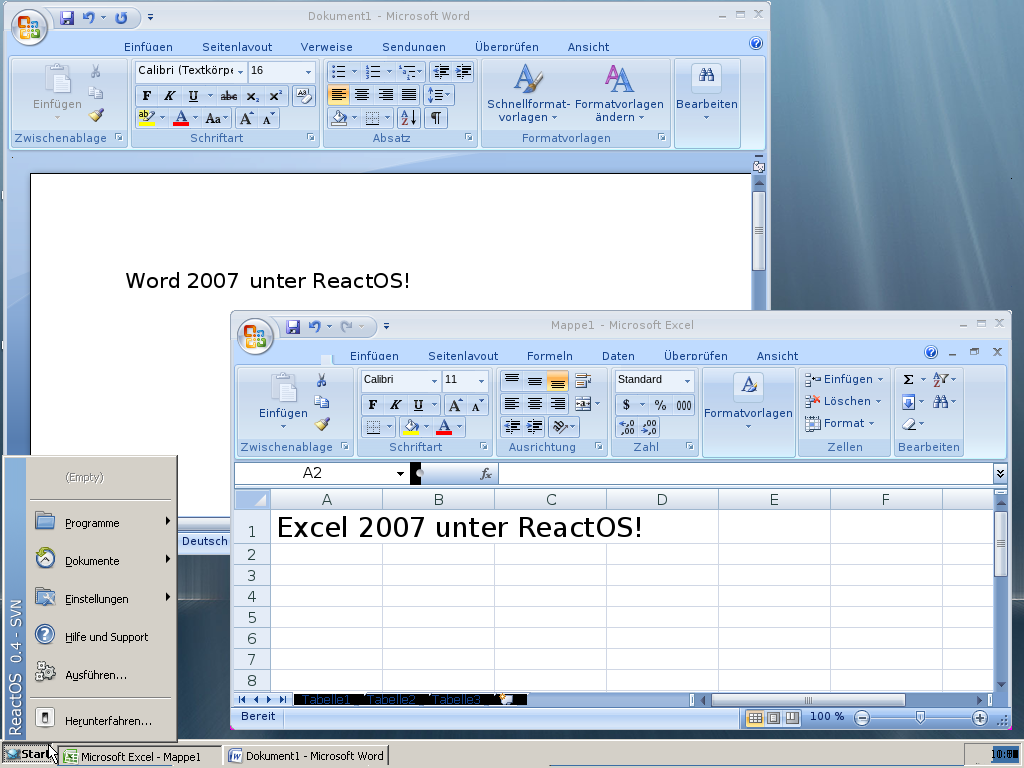
\includegraphics{pictures/office2007ros}
\end{frame}

\subsection{Technical Terms}
\begin{frame}{Technical Terms}
	\begin{itemize}
		\item \textbf{API} \\
					Official and documented interface to let a software developer make use of a component
					\bigskip
					
		\item \textbf{GDI} \\
					Windows component for drawing text and graphics on the screen and on paper
					\bigskip
					
		\item \textbf{Spooler} \\
					Buffers concurrent print requests from multiple applications and sends them,\\
					one after another, to the Printer
					\bigskip
	\end{itemize}
\end{frame}

\subsection{Microsoft Windows Printing Stack}
\begin{frame}{Microsoft Windows Printing Stack}
	\centering
	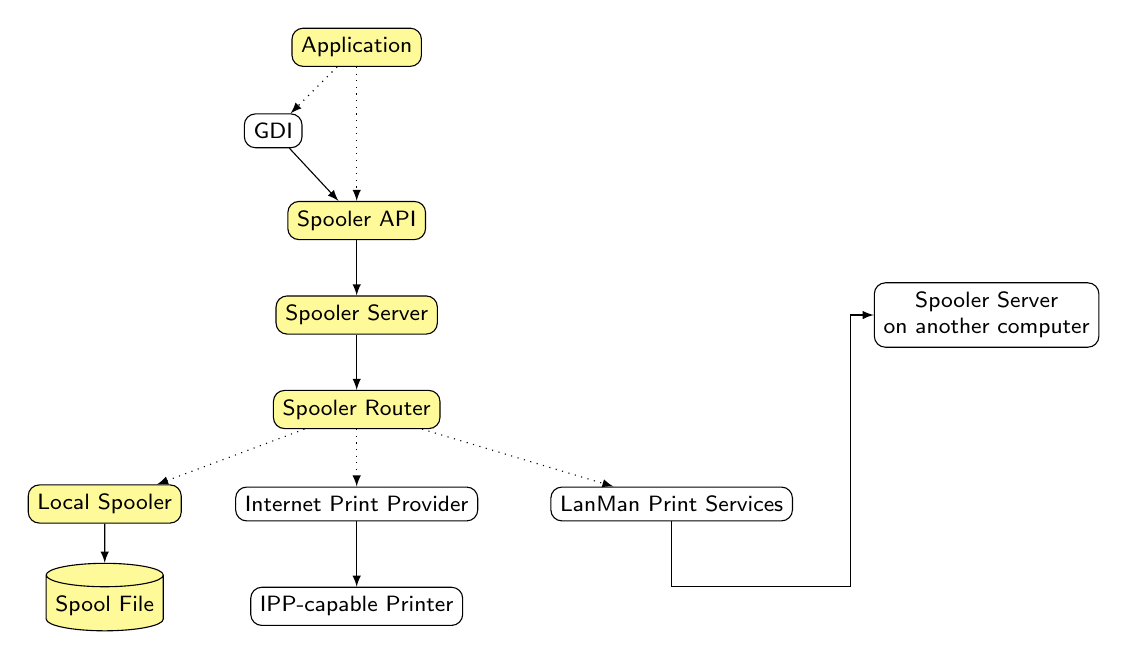
\begin{tikzpicture}
		\node [cf_block, cf_impl] (App) {Application};
		\node [cf_block, below left = 15mm of App] (gdi32) {GDI};
		\node [cf_block, cf_impl, below = 22mm of App] (winspool) {Spooler API};
		\path [cf_line, dotted] (App) -- (gdi32);
		\path [cf_line, dotted] (App) -- (winspool);
		\path [cf_line] (gdi32) -- (winspool);
				
		\uncover<2->{
			\node [cf_block, cf_impl, below = of winspool] (spoolsv) {Spooler Server};
			\path [cf_line] (winspool) -- (spoolsv);
		}
		
		\uncover<3->{
			\node [cf_block, cf_impl, below = of spoolsv] (spoolss) {Spooler Router};
			\path [cf_line] (spoolsv) -- (spoolss);
		}
		
		\uncover<4->{
			\node [cf_block, cf_impl, below left = 12mm and 32mm of spoolss] (localspl) {Local Spooler};
			\node [cf_block, below = of spoolss] (inetpp) {Internet Print Provider};
			\node [cf_block, below right = 12mm and 40mm of spoolss] (win32spl) {LanMan Print Services};
			\path [cf_line, dotted] (spoolss) -- (localspl);
			\path [cf_line, dotted] (spoolss) -- (inetpp);
			\path [cf_line, dotted] (spoolss) -- (win32spl);
		}
		
		\uncover<5->{
			\node [cf_block, right = 80mm of spoolsv] (extern_spoolsv) {Spooler Server\\on another computer};
			\node [cf_data, cf_impl, below = 13mm of localspl] (spoolfile) {Spool File};
			\node [cf_block, below = 13mm of inetpp] (ippprinter) {IPP-capable Printer};
			
			\path [cf_line] (localspl) -- (spoolfile);
			\path [cf_line] (inetpp) -- (ippprinter);
			
			\coordinate [left = 3mm of extern_spoolsv] (extern_spoolsv_anchor);
			\path [draw] (win32spl) -- (win32spl |- ippprinter.north);
			\path [draw] (win32spl |- ippprinter.north) -- (ippprinter.north -| extern_spoolsv_anchor);
			\path [draw] (ippprinter.north -| extern_spoolsv_anchor) -- (extern_spoolsv_anchor);
			\path [cf_line] (extern_spoolsv_anchor) -- (extern_spoolsv.west);
		}
	\end{tikzpicture}
	
	\begin{tikzpicture}[remember picture, overlay]
		\node [cf_base, align=right, xshift=130mm, yshift=-13mm] at (titleAnchor) {Implemented components\\in \colorbox{yellow!40}{yellow}};
	\end{tikzpicture}
\end{frame}

\begin{frame}{Microsoft Windows Printing Stack}
	\centering
	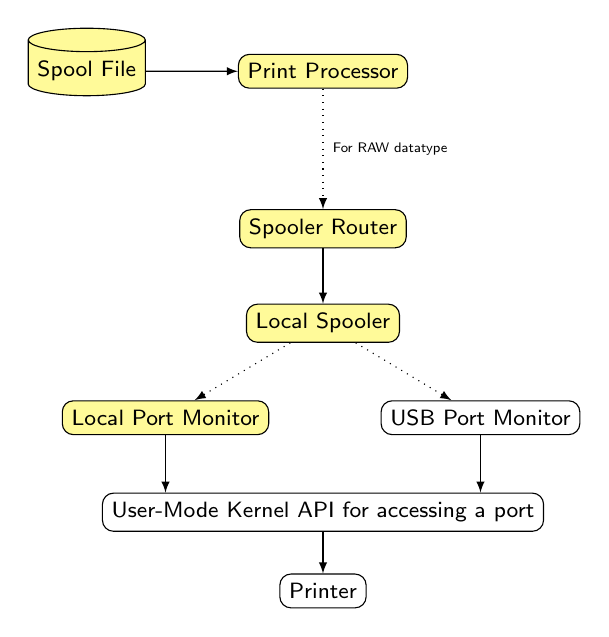
\begin{tikzpicture}
		\node [cf_data, cf_impl] (spoolfile) {Spool File};
		\node [cf_block, cf_impl, right = 30mm of spoolfile] (winprint) {Print Processor};
		\path [cf_line] (spoolfile.east) -- (winprint.west);
		
		\uncover<2->{
			\node [cf_block, cf_impl, below = 20mm of winprint] (spoolss) {Spooler Router};
			\node [cf_block, cf_impl, below = of spoolss] (localspl) {Local Spooler};
			\path [cf_line, dotted] (winprint) -- (spoolss);
			\path [cf_label] (winprint) edge node [right] {For RAW datatype} (spoolss);
			\path [cf_line] (spoolss) -- (localspl);
		}
		
		\uncover<3->{
			\node [cf_block, cf_impl, below left = 12mm and 20mm of localspl] (localmon) {Local Port Monitor};
			\node [cf_block, below right = 12mm and 20mm of localspl] (usbmon) {USB Port Monitor};
			\path [cf_line, dotted] (localspl) -- (localmon);
			\path [cf_line, dotted] (localspl) -- (usbmon);
		}
		
		\uncover<4->{
			\node [cf_block, below = 24mm of localspl] (kernel32) {User-Mode Kernel API for accessing a port};
			\node [cf_block, below = 10mm of kernel32] (printer) {Printer};
			\path [cf_line] (localmon) -- (kernel32.north -| localmon);
			\path [cf_line] (usbmon) -- (kernel32.north -| usbmon);
			\path [cf_line] (kernel32) -- (printer);
		}
	\end{tikzpicture}
	
	\begin{tikzpicture}[remember picture, overlay]
		\node [cf_base, align=right, xshift=130mm, yshift=-13mm] at (titleAnchor) {Implemented components\\in \colorbox{yellow!40}{yellow}};
	\end{tikzpicture}
\end{frame}

\subsection{Remote Procedure Calls (RPC)}
\begin{frame}{Remote Procedure Calls (RPC)}
	\myheading{Call a function in another process, on another computer}
	
	Here used for Spooler API $\rightarrow$ Spooler Server communication.
	\bigskip
	
	\begin{itemize}
		\item Function call and parameter information are transmitted over the network
		\item No network-specific code needs to be written
	\end{itemize}
	
	\bigskip
	\pause
	
	Remote function call as easy as a local one!
	
	\bigskip
	
	Example:\\
	\footnotesize\texttt{\_RpcOpenPrinter(L"\textbackslash\textbackslash\textbackslash\textbackslash Computer\textbackslash\textbackslash Printer", \&hPrinter, Datatype, \&DevMode, AccessRequired);}
\end{frame}

\begin{frame}{Remote Procedure Calls (RPC)}
	What's happening in the background:

	\begin{enumerate}
		\item \textbf{Marshalling:} Function name and parameters are packed into a message.
		\item Message is transmitted over the network.
		\item \textbf{Unmarshalling:} Function name and parameters are reconstructed out of the message.
		\item The actual implemented function is called in the target application.
	\end{enumerate}
\end{frame}

\section{Methods}

\subsection{Reverse Engineering Tools}
\begin{frame}{Reverse Engineering Tools}
	\centering
	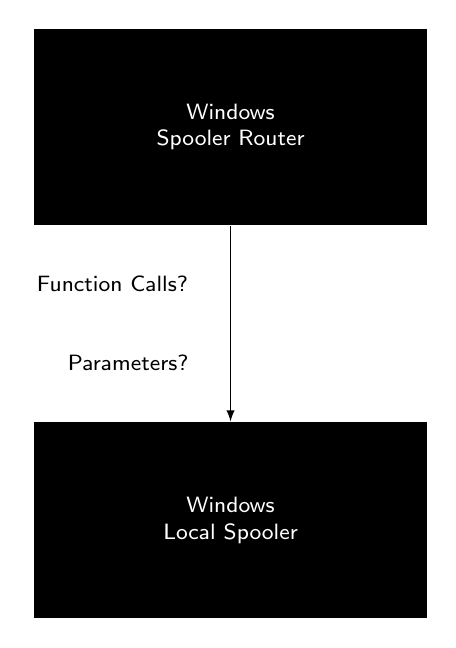
\begin{tikzpicture}
		\node [cf_blackbox] (spoolss) {Windows\\Spooler Router};
		\node [cf_blackbox, below = 50mm of spoolss] (localspl) {Windows\\Local Spooler};
		\path [cf_line] (spoolss) -- (localspl);
		
		\node [cf_base, on grid, below left = 20mm and 15mm of spoolss] {Function Calls?};
		\node [cf_base, on grid, below left = 30mm and 13mm of spoolss] {Parameters?};
	\end{tikzpicture}
\end{frame}

\begin{frame}{Reverse Engineering Tools}
	\myheading{Dependency Walker}
	
	Reveals dependencies between modules and their imported and exported functions
	\bigskip
	
	\centering
	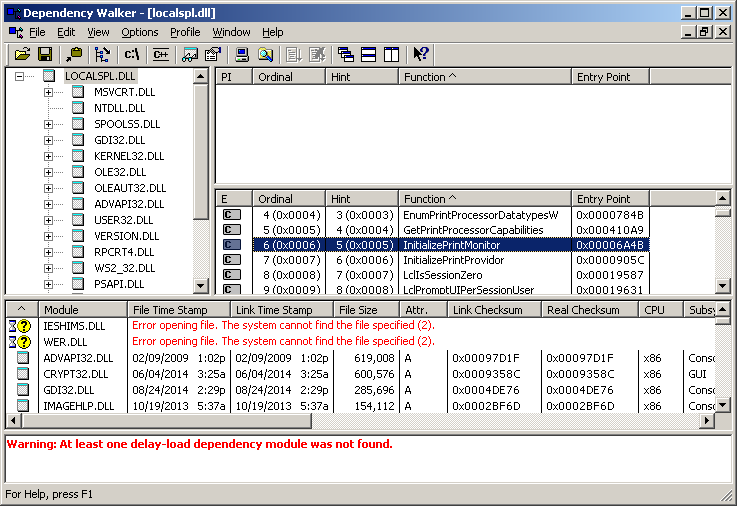
\includegraphics{pictures/depends}
	
	\begin{tikzpicture}[remember picture, overlay]
		\node<2-> [cf_base, align=center, xshift=15mm, yshift=-30mm] at (titleAnchor) {Examining\\ \colorbox{windows_gray}{Local Spooler}};	
		\node<3-> [cf_base, align=center, xshift=138mm, yshift=-51mm] at (titleAnchor) {Found function\\ \colorbox{windows_blue}{\textcolor{white}{InitializePrintMonitor}}};
	\end{tikzpicture}
\end{frame}

\begin{frame}{Reverse Engineering Tools}
	\myheading{GNU strings}
	
	Outputs all strings found in a binary file
	\bigskip
	
	\centering
	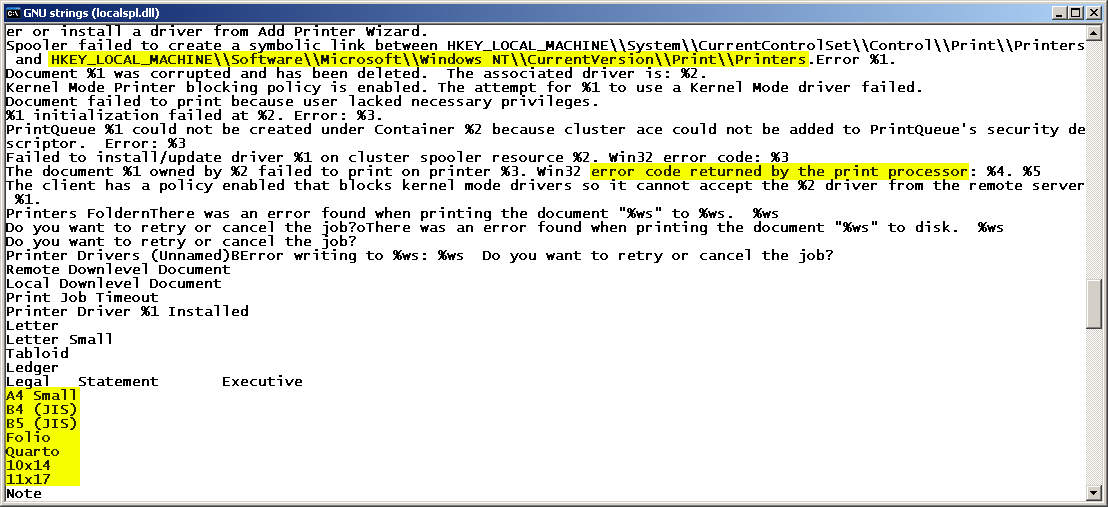
\includegraphics{pictures/strings}
\end{frame}

\begin{frame}{Reverse Engineering Tools}
	\myheading{API Monitor}
	
	Monitors all calls done to system functions and their parameters
	\bigskip
	
	\centering
	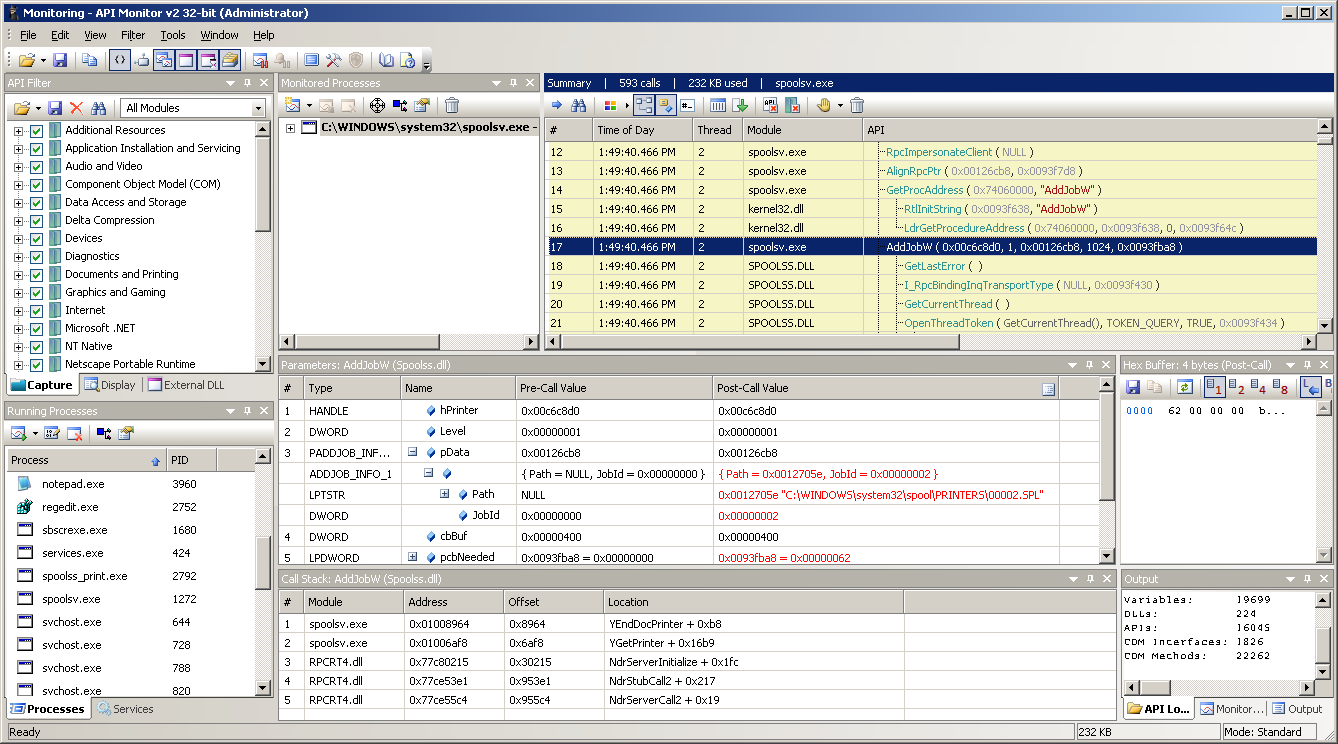
\includegraphics{pictures/apimon}
\end{frame}

\begin{frame}{Reverse Engineering Tools}
	\centering
	\begin{tikzpicture}
		\node [cf_blackbox] (spoolss) {Windows\\Spooler Router};
		\node [cf_blackbox, below = 50mm of spoolss] (localspl) {Windows\\Local Spooler};
		\path [cf_line] (spoolss) -- (localspl);
		
		\node [cf_base, on grid, below left = 20mm and 15mm of spoolss] {Function Calls?};
		\node [cf_base, on grid, below left = 30mm and 13mm of spoolss] {Parameters?};
		
		\node [cf_block, below = 8mm of localspl] {$\vcenter{\hbox{
\includegraphics[height=2ex]{pictures/glass}}}$ GNU strings};
		\node [cf_block, below right = 20mm and 20mm of spoolss] {$\vcenter{\hbox{
\includegraphics[height=2ex]{pictures/glass}}}$ Dependency Walker};
		\node [cf_block, below right = 30mm and 15mm of spoolss] {$\vcenter{\hbox{
\includegraphics[height=2ex]{pictures/glass}}}$ API Monitor};
	\end{tikzpicture}
\end{frame}

\section{Implementation}

\subsection{Skip Lists}
\begin{frame}{Skip Lists}
	\centering
	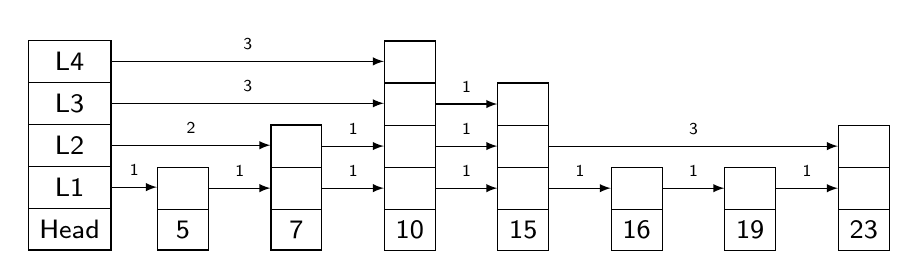
\begin{tikzpicture}[scale=1.2, every node/.append style={transform shape}]
		\node[cf_skiplistitem=5] (H) {L4 \nodepart{two} L3 \nodepart{three} L2 \nodepart{four} L1 \nodepart{five} Head};
		\node[cf_skiplistitem=2, right = of H.south, anchor = south] (5) {\nodepart{two} 5};
		\node[cf_skiplistitem=3, right = of 5.south, anchor = south] (7) {\nodepart{three} 7};
		\node[cf_skiplistitem=5, right = of 7.south, anchor = south] (10) {\nodepart{five} 10};
		\node[cf_skiplistitem=4, right = of 10.south, anchor = south] (15) {\nodepart{four} 15};
		\node[cf_skiplistitem=2, right = of 15.south, anchor = south] (16) {\nodepart{two} 16};
		\node[cf_skiplistitem=2, right = of 16.south, anchor = south] (19) {\nodepart{two} 19};
		\node[cf_skiplistitem=3, right = of 19.south, anchor = south] (23) {\nodepart{three} 23};
		
		\path [cf_line, cf_onslide=<2->{draw=red, cf_emphline}] (H.one east) -- (10.one west |- H.one east);
		\path [cf_line] (H.two east) -- (10.two west |- H.two east);
		\path [cf_line] (H.three east) -- (7.one west |- H.three east);
		\path [cf_line, cf_onslide=<3->{draw=blue, cf_emphline}] (H.four east) -- (5.one west |- H.four east);
		\path [cf_line, cf_onslide=<3->{draw=blue, cf_emphline}] (5.one east) -- (7.two west |- 5.one east);
		\path [cf_line] (7.one east) -- (10.three west |- 7.one east);
		\path [cf_line, cf_onslide=<3->{draw=blue, cf_emphline}] (7.two east) -- (10.four west |- 7.two east);
		\path [cf_line, cf_onslide=<2->{draw=red, cf_emphline}] (10.two east) -- (15.one west |- 10.two east);
		\path [cf_line] (10.three east) -- (15.two west |- 10.three east);
		\path [cf_line, cf_onslide=<3->{draw=blue, cf_emphline}] (10.four east) -- (15.three west |- 10.four east);
		\path [cf_line] (15.two east) -- (23.one west |- 15.two east);
		\path [cf_line] (15.three east) -- (16.one west |- 15.three east);
		\path [cf_line] (16.one east) -- (19.one west |- 16.one east);
		\path [cf_line] (19.one east) -- (23.two west |- 19.one east);
		
		\path [cf_label, cf_onslide=<4->{red}] (H.one east) edge node [above] {3} (10.one west |- H.one east);
		\path [cf_label] (H.two east) edge node [above] {3} (10.two west |- H.two east);
		\path [cf_label] (H.three east) edge node [above] {2} (7.one west |- H.three east);
		\path [cf_label] (H.four east) edge node [above] {1} (5.one west |- H.four east);
		\path [cf_label] (5.one east) edge node [above] {1} (7.two west |- 5.one east);
		\path [cf_label] (7.one east) edge node [above] {1} (10.three west |- 7.one east);
		\path [cf_label] (7.two east) edge node [above] {1} (10.four west |- 7.two east);
		\path [cf_label, cf_onslide=<4->{red}] (10.two east) edge node [above] {1} (15.one west |- 10.two east);
		\path [cf_label] (10.three east) edge node [above] {1} (15.two west |- 10.three east);
		\path [cf_label] (10.four east) edge node [above] {1} (15.three west |- 10.four east);
		\path [cf_label] (15.two east) edge node [above] {3} (23.one west |- 15.two east);
		\path [cf_label] (15.three east) edge node [above] {1} (16.one west |- 15.three east);
		\path [cf_label] (16.one east) edge node [above] {1} (19.one west |- 16.one east);
		\path [cf_label] (19.one east) edge node [above] {1} (23.two west |- 19.one east);
	\end{tikzpicture}
	
	\bigskip
	
	\begin{itemize}
		\item Fast insertions, deletions and lookups, \\ $\mathcal{O}(\log n)$ on average
		\item Easy to implement
		\item Extensible
	\end{itemize}
\end{frame}

\begin{frame}{Skip Lists}
	\myheading{Example: Data Structure with 1000 Elements}
	\vspace{15mm}
	
	\centering
	\large Average Number Of Comparisons During A Lookup
	\vspace{10mm}
	
	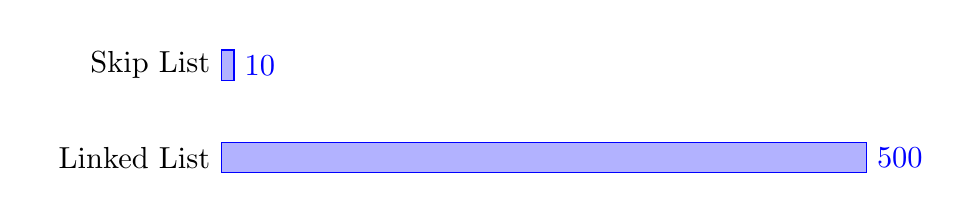
\begin{tikzpicture}[scale=1.1]
		\begin{axis}[
			xbar,
			xmin = 0,
			width = 100mm,
			height = 35mm,
			enlarge x limits = {rel=0.13, upper},
			ytick = {1,2},
			yticklabels = {Linked List, Skip List},
			enlarge y limits = 0.4,
			nodes near coords,
			y axis line style = { opacity = 0 },
			axis x line = none,
			tickwidth = 0
		]
			\addplot coordinates {(500,1) (10,2)};
		\end{axis}
	\end{tikzpicture}
	
	\vspace{15mm}
\end{frame}

%%
%% the final slide (contact information) can be generated with the following
%% command
%%
\lastpage

\end{document}
